\documentclass{article}
\usepackage{tikz}

\begin{document}

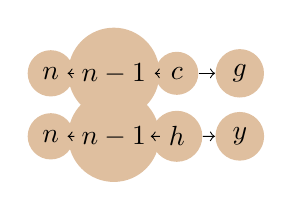
\begin{tikzpicture}[scale=0.8]
    % Nodes
    \node at (0, 0) [circle, fill=brown!50] (n) {$n$};
    \node at (1, 0) [circle, fill=brown!50] (n_minus_1) {$n-1$};
    \node at (2, 0) [circle, fill=brown!50] (c) {$c$};
    \node at (3, 0) [circle, fill=brown!50] (g) {$g$};
    
    \node at (0, -1) [circle, fill=brown!50] (n_below) {$n$};
    \node at (1, -1) [circle, fill=brown!50] (n_minus_1_below) {$n-1$};
    \node at (2, -1) [circle, fill=brown!50] (h) {$h$};
    \node at (3, -1) [circle, fill=brown!50] (y) {$y$};

    % Edges
    \draw[->] (n) -- (n_minus_1);
    \draw[->] (n_minus_1) -- (c);
    \draw[->] (c) -- (g);
    
    \draw[->] (n_below) -- (n_minus_1_below);
    \draw[->] (n_minus_1_below) -- (h);
    \draw[->] (h) -- (y);
\end{tikzpicture}

\end{document}